% !TeX spellcheck = ru_RU
% !TeX encoding = UTF-8
\subsection{Общая структурная схема и план описания системы}
\subsubsection{Общая структурная схема}\label{7.1}
В данном подразделе мы рассмотрим общую структурную схему системы. Данная общая схема отражает основные особенности реальных систем, которые будут рассмотрены в последующих разделах.
Общая структурная схема системы представлена на рисунке 
\ref{fig:common_chart}.

\begin{figure}[h]
	\centering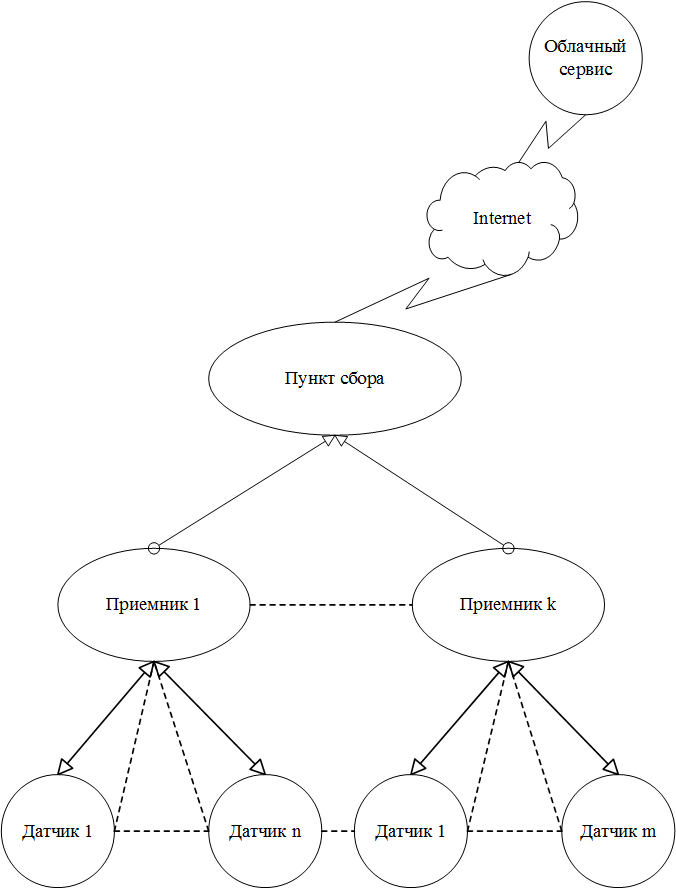
\includegraphics[width=0.7\linewidth]{img/common_chart}
	\caption{Общая структурная схема системы}
	\label{fig:common_chart}
\end{figure}

В системе имеются следующие компоненты: 
\begin{itemize}
	\item "Датчики".
	\item "Приёмники". 
	\item "Пункт сбора".
	\item Облачный сервер.
\end{itemize}

Под "датчиком" будем понимать устройство, которое включает в себя некоторый сенсор (например, термо-датчик, датчик освещенности и т.п.) и передающее устройство. В некоторых случаях "датчик" может содержать не только передающее, но и принимающее устройство. Кроме того, иногда "датчик" может содержать не только сенсор, но и некоторый исполнительный механизм (например, сервопривод). Под "приёмником" будем понимать устройство, которое принимает данные от нескольких "датчиков", делает некоторую обработку и передает эти данные далее на "пункт сбора". В некоторых случаях "приёмник" может принимать данные от "пункта сбора" и передавать их "датчикам".

В общем случае работу системы можно описать следующим образом. Данные от "датчиков" по определенному протоколу передаются "приёмником".
На одном "приёмнике" принимаются данные от нескольких "датчиков" и предварительно обрабатываются. Данные от "приёмников" по определенному протоколу передаются на "пункт сбора", где производится дальнейшая обработка этих данных. С "пункта сбора" данные по протоколу TCP/IP или UDP/IP через интернет передаются в некоторый облачный сервер.

В некоторых случаях от "пункта сбора" на "приёмник" могут передаваться данные, которые далее "приёмник" передает на "датчики"(например, это управляющие команды, которые производят настройку сенсоров и т.п).  
\subsubsection{План описания системы}
Каждую систему будем описывать по следующему плану:
\begin{itemize}
	\item Назначение системы.
	\item Структура системы. 
	\item Разбиение системы на уровни.
	\item Особенности построения уровней.
\end{itemize}
При описании назначения системы необходимо указать область применения данной системы, частотный радиодиапазон, в котором работает система, стандарты, на основе которых построена данная система и т.п. Кроме того, при описании назначения системы, необходимо дать ссылки на источники, где описана данная система. 

Рассказывая о структуре системы необходимо показать, как соотносится структура системы с общей структурной схемой системы,
описанной в разделе \ref{7.1}.
и указать, возможна ли в данной системе передача данных от "приемников" к "датчикам".    

Описывая  разбиение системы на уровни, необходимо дать краткое описание каждого уровня и указать, является ли данный уровень открытым или нет.

Если у системы есть специфические особенности построения некоторых уровней, то их необходимо описать и дать ссылки на источники, где имеется подробное описание этих особенностей.
